\begin{frame}{Methods}

\begin{backgroundblock}{30mm}{5mm}
	\begin{tikzpicture}[framed,background rectangle/.style={thick, rounded corners, draw=black}]
		\node[inner sep=1pt] (screen) at (10,-5)
    		{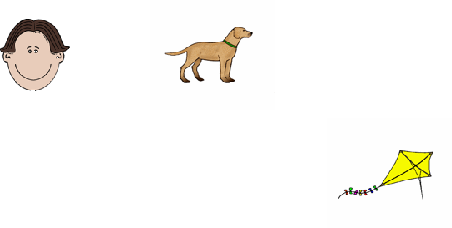
\includegraphics[scale=.5]{gfx/method/build/screen-3}};   		
    		\node[font = \tiny, below = 0cm of screen] {Condition 1: A and B moved above C};
	\end{tikzpicture}
\end{backgroundblock}

\begin{backgroundblock}{75mm}{5mm}
	\begin{tikzpicture}[framed,background rectangle/.style={thick, rounded corners, draw=black}]
		\node[inner sep=3.5pt] (screen) at (10,-5)
    		{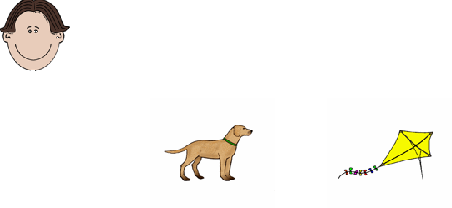
\includegraphics[scale=.5]{gfx/method/build/screen-4}};   			    					\node[font = \tiny, below = 0cm of screen] {Condition 2: A moved above B and C};
	\end{tikzpicture}
\end{backgroundblock}

\vspace{2cm}
\begin{footnotesize}
\begin{minipage}[t]{.4\textwidth}
	\begin{itemize}
		\item \uncover<2->{48 items; 96 fillers; 6 practice trials}
		\item \uncover<2->{First noun: \textit{Peter} or \textit{Tania}}
		%	\item \uncover<4>{Movement: up or down}
		\item \uncover<2->{Image names: high frequency and naming agreement.}
	\end{itemize}
\end{minipage}
\hfill
\begin{minipage}[t]{.525\textwidth}
\setlength{\leftmargini}{0.5cm}
\setlength{\leftmarginii}{0.5cm}
\begin{itemize}
	\item \textbf{Experiment 1:}
	\begin{itemize}
		\item[1a.] \uncover<3->{\textbf{Peter and the dog} moved above the kite}
		\item[1b.] \uncover<3->{\textbf{Peter} moved above the dog and the kite}
		\item \uncover<3->{78 ppts (after cleaning)}
	\end{itemize}
	\item \textbf{Experiment 2:}
	\begin{itemize}
		\item[2.] \uncover<4->{Peter, the dog, the kite}
		\item \uncover<4->{45 ppts (after cleaning)}
	\end{itemize}
\end{itemize}
\end{minipage}
\end{footnotesize}

\end{frame}